\documentclass[11pt, fleqn]{article}

\usepackage[usenames,dvipsnames,svgnames,table]{xcolor}
\usepackage{amsmath}
\usepackage{amsfonts}
\usepackage[margin=1in]{geometry} % To set the margin widths
\usepackage{graphicx}
\usepackage{listings}
\usepackage{multirow}
\usepackage{tabularx}
\usepackage{varioref}
\usepackage[noabbrev,capitalize]{cleveref}
\usepackage[group-separator={,}]{siunitx}
\usepackage{subcaption}
\usepackage{titlesec}
\usepackage{lscape}
\usepackage{bm}
\usepackage{chngpage}
\usepackage[titletoc,toc,title]{appendix}

\renewcommand\thesection{\arabic{section}}
\renewcommand\thesubsection{\thesection\alph{subsection}}

\lstset{
  frame=single,
  basicstyle=\ttfamily,% print whole listing small
  language=R,
  aboveskip=3mm,
  belowskip=3mm,
  showstringspaces=false,
  columns=flexible,
  numbers=none,
  commentstyle=\color{ForestGreen},
  stringstyle=\color{Maroon},
  breaklines=true,
  breakatwhitespace=true,
  tabsize=2,
  literate={<-}{{$\gets$}}1 {~}{{$\sim$}}1
}

\sisetup{output-exponent-marker=\textsc{e}}

\setlength{\parskip}{12pt} % Sets a blank line in between paragraphs
\setlength\parindent{0pt} % Sets the indent for each paragraph to zero

\begin{document}

\title{Homework \#1\\
Digital and Algorithmic Marketing (37304-01)}
\author{Brian Chingono, Will Clark, Matthew DeLio, Yoni Sarason, Jonathan Stevens\\
University of Chicago Booth School of Business}

\maketitle

\section{Data Exploration (JS)}

% Note this CDF plot is for customers that did spend at least something
\begin{figure}[!htb]
  \centering
  \caption{CDF of Customer Spending}
  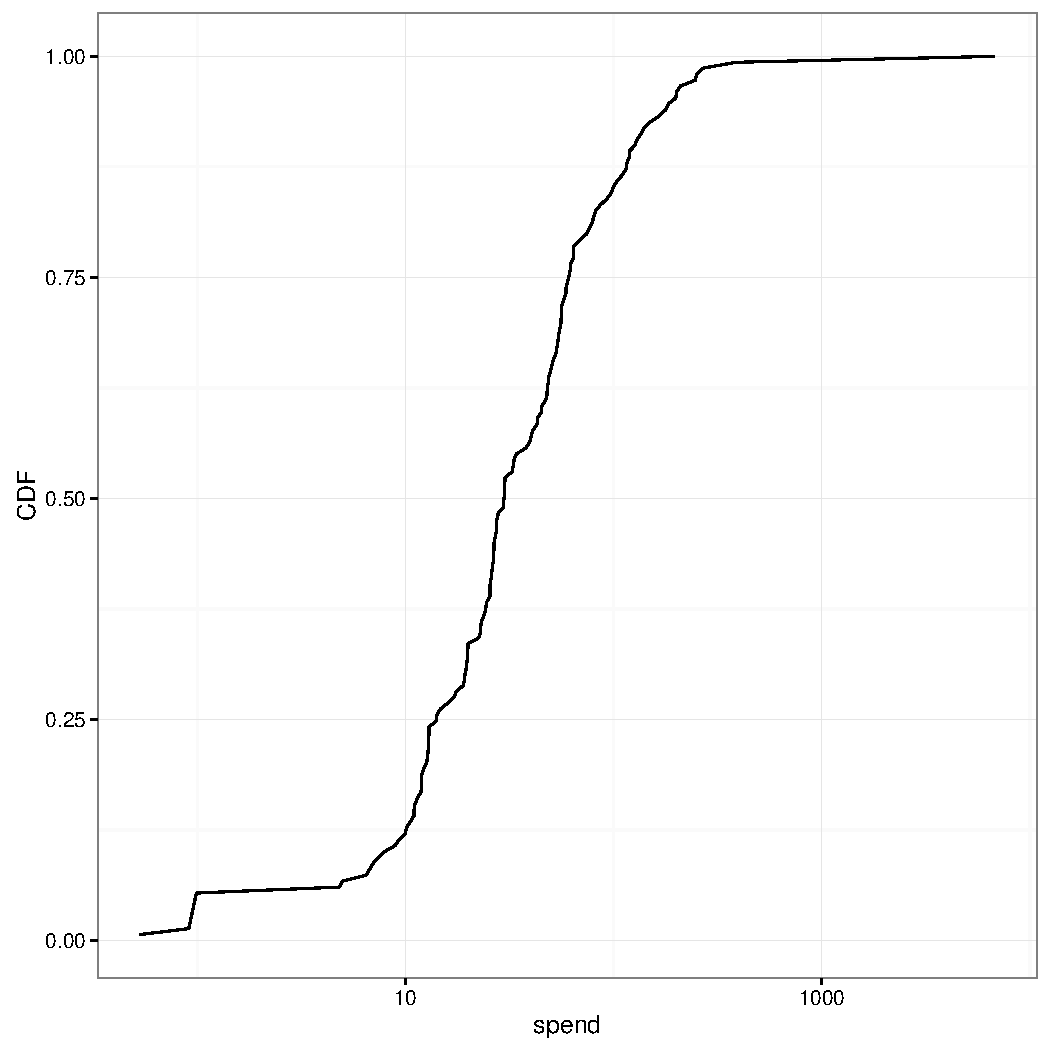
\includegraphics[scale=.5]{cust_spend_cdf.pdf}
  \label{fig:cust_spend_cdf}
\end{figure}

% Again, this is for actual customers that spent something.
% we might want to only include the histogram or cdf.
\begin{figure}[!htb]
  \centering
  \caption{Histogram of Customer Spending}
  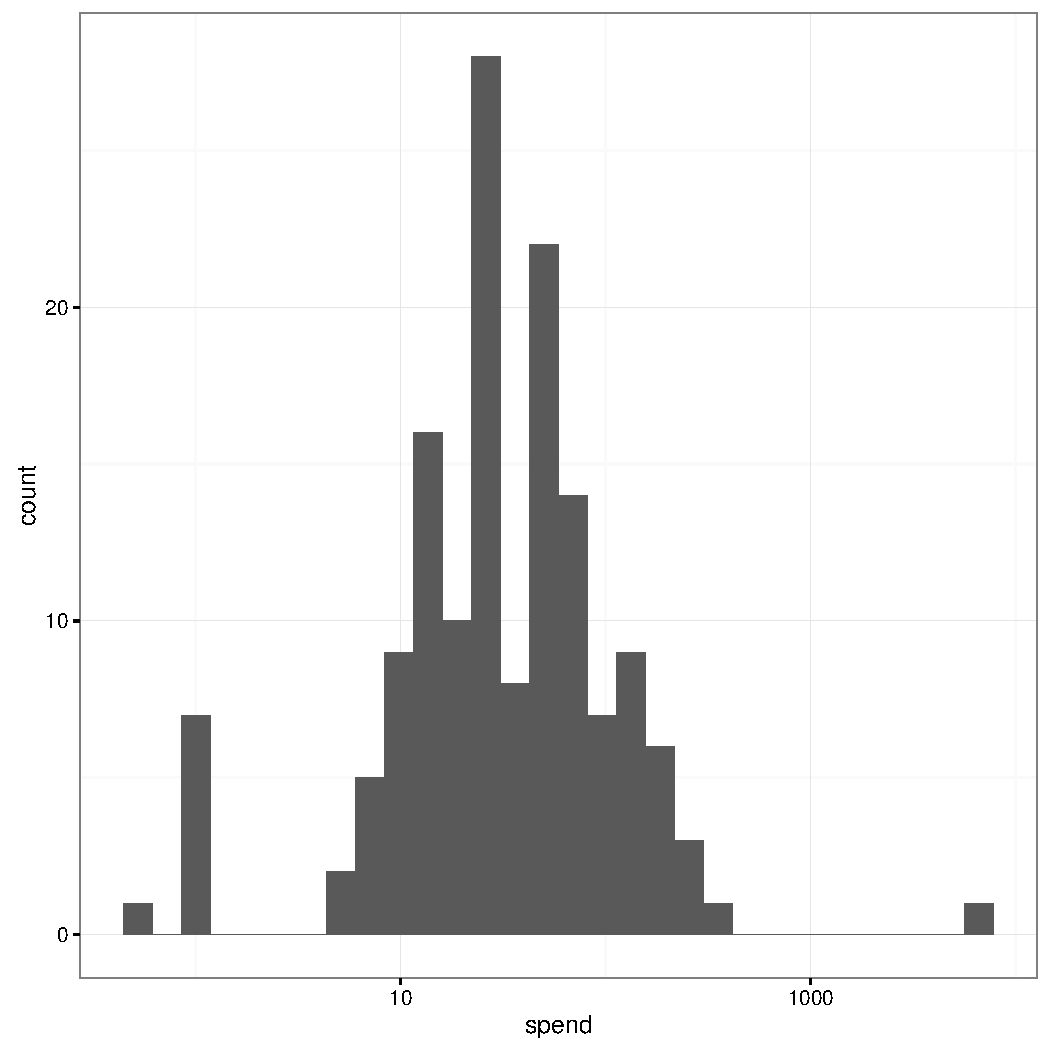
\includegraphics[scale=.5]{cust_spend_hist.pdf}
  \label{fig:cust_spend_hist}
\end{figure}


\section{K-Means Matching (WC)}

We first built a matching algorithm using k-means clustering. We used the following algorithm:
\begin{itemize}
\item Find every fifth quantile of non-zero customer spending (see \cref{tab:cutoffs} in the Appendix). We will define a valuable customer as one who spends at or above the quantile level. For each quantile:
\begin{itemize}
\item Use a k-means algorithm to break the customers into $k$ clusters, where we search over a range of $k$ from 1 to 20. For each $k$ number of clusters:
\begin{itemize}
\item Define the "matching" group in the target set as the nearest $j$ clusters, where we vary $j$ from 1 to $k$. For example, suppose that we use $k=10$ clusters. Then we would define the "match" data set as the nearest cluster, then the nearest two clusters, then the nearest three clusters, etc.
\end{itemize}
\end{itemize}
\item For each combination of the quantile cutoff, $k$ clusters, and $j$ matches, calculate the profitability of targeting the resulting match data set. The optimal set of parameters is that which maximizes profitability.
\end{itemize}
We use this algorithm to find the most profitable targeting strategy in the original data set and the data set that includes the ecom\_index. \textbf{In both cases, the algorithm fails to produce a profitable strategy.}

\section{K-Nearest-Neighbors Matching (MLD)}

% latex table generated in R 3.2.3 by xtable 1.8-2 package
% Tue Apr 12 04:02:36 2016
\begin{table}[ht]
\centering
\caption{Significant Coefficients by Series} 
\label{tab:series_coefs}
\begin{tabular}{rlll}
  \hline
 & No ecom\_index (BIC) & With ecom\_index (BIC) & With ecom\_index (AIC) \\ 
  \hline
1 & census\_region2 & census\_region2 & census\_region2 \\ 
  2 & household\_size6 & household\_size6 & household\_size6 \\ 
  3 & hoh\_oldest\_age2 & hoh\_oldest\_age2 & hoh\_oldest\_age2 \\ 
  4 & household\_income6 & household\_income6 & household\_income6 \\ 
  5 & retail\_index & ecom\_index & retail\_index \\ 
  6 &  &  & ecom\_index \\ 
   \hline
\end{tabular}
\end{table}


% latex table generated in R 3.2.3 by xtable 1.8-2 package
% Tue Apr 12 03:01:59 2016
\begin{table}[ht]
\centering
\caption{Best matching threshold by explanatory variables} 
\label{tab:series_max}
\begin{tabular}{lrlrrrrr}
  \hline
Series & MatchingThreshold [\$] & Threshold \% & Best NN Choice & Profit [\$] & \% Cust Captured & \% Revenue Captured & \% Cust Matched \\ 
  \hline
Manual & 41.10 & 57.5\% &   7 & 4800.48 & 79.09 & 82.79 & 43.72 \\ 
  AIC & 8.72 & 10\% &   3 & 5028.85 & 82.73 & 85.17 & 51.41 \\ 
  BIC & 35.62 & 55\% &   7 & 4541.70 & 76.36 & 80.04 & 37.67 \\ 
   \hline
\end{tabular}
\end{table}


\begin{figure}[!htb]
  \centering
  \caption{Max Profits by Series and Threshold}
  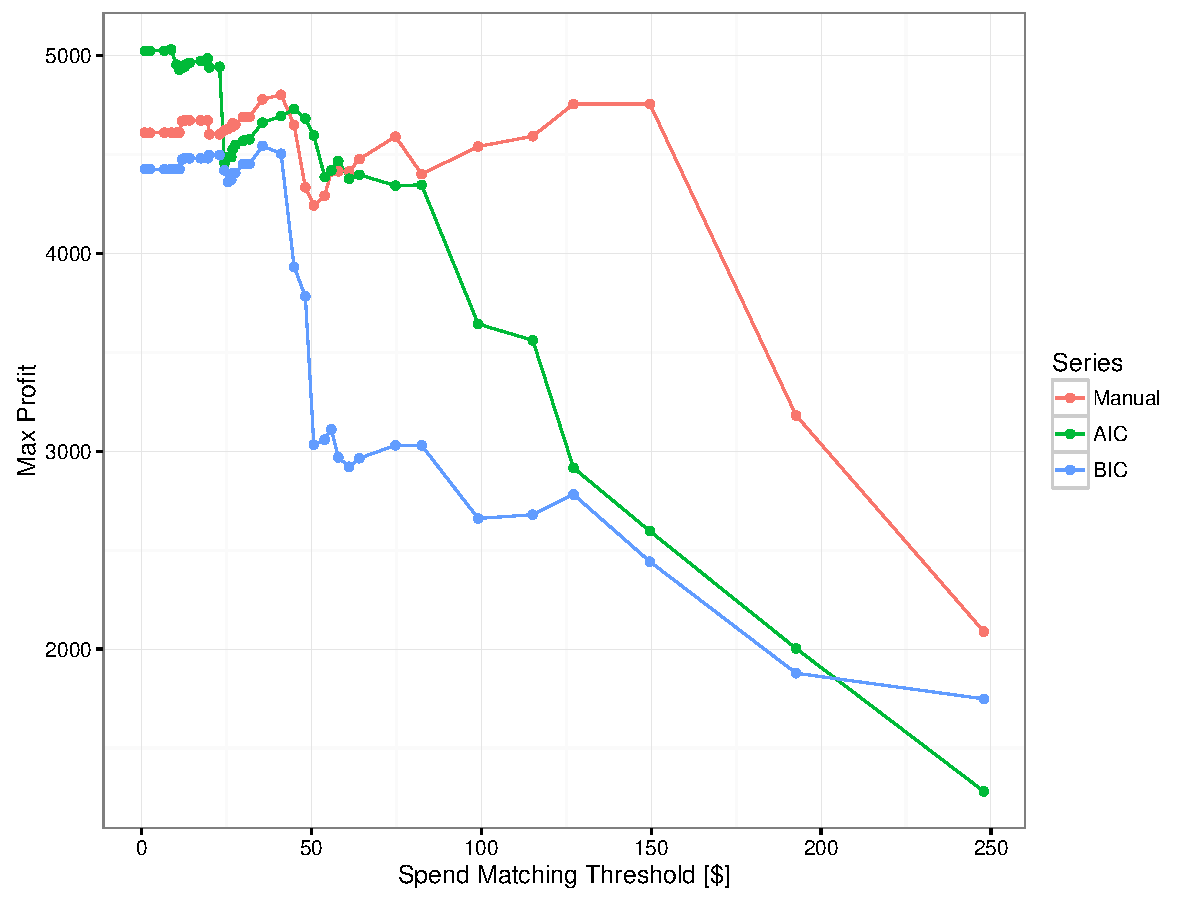
\includegraphics[scale=.5]{threshold_max_profit.pdf}
  \label{fig:threshold_max_profit}
\end{figure}

\begin{figure}[!htb]
  \centering
  \caption{Profits using K-Nearest Neighbors}
  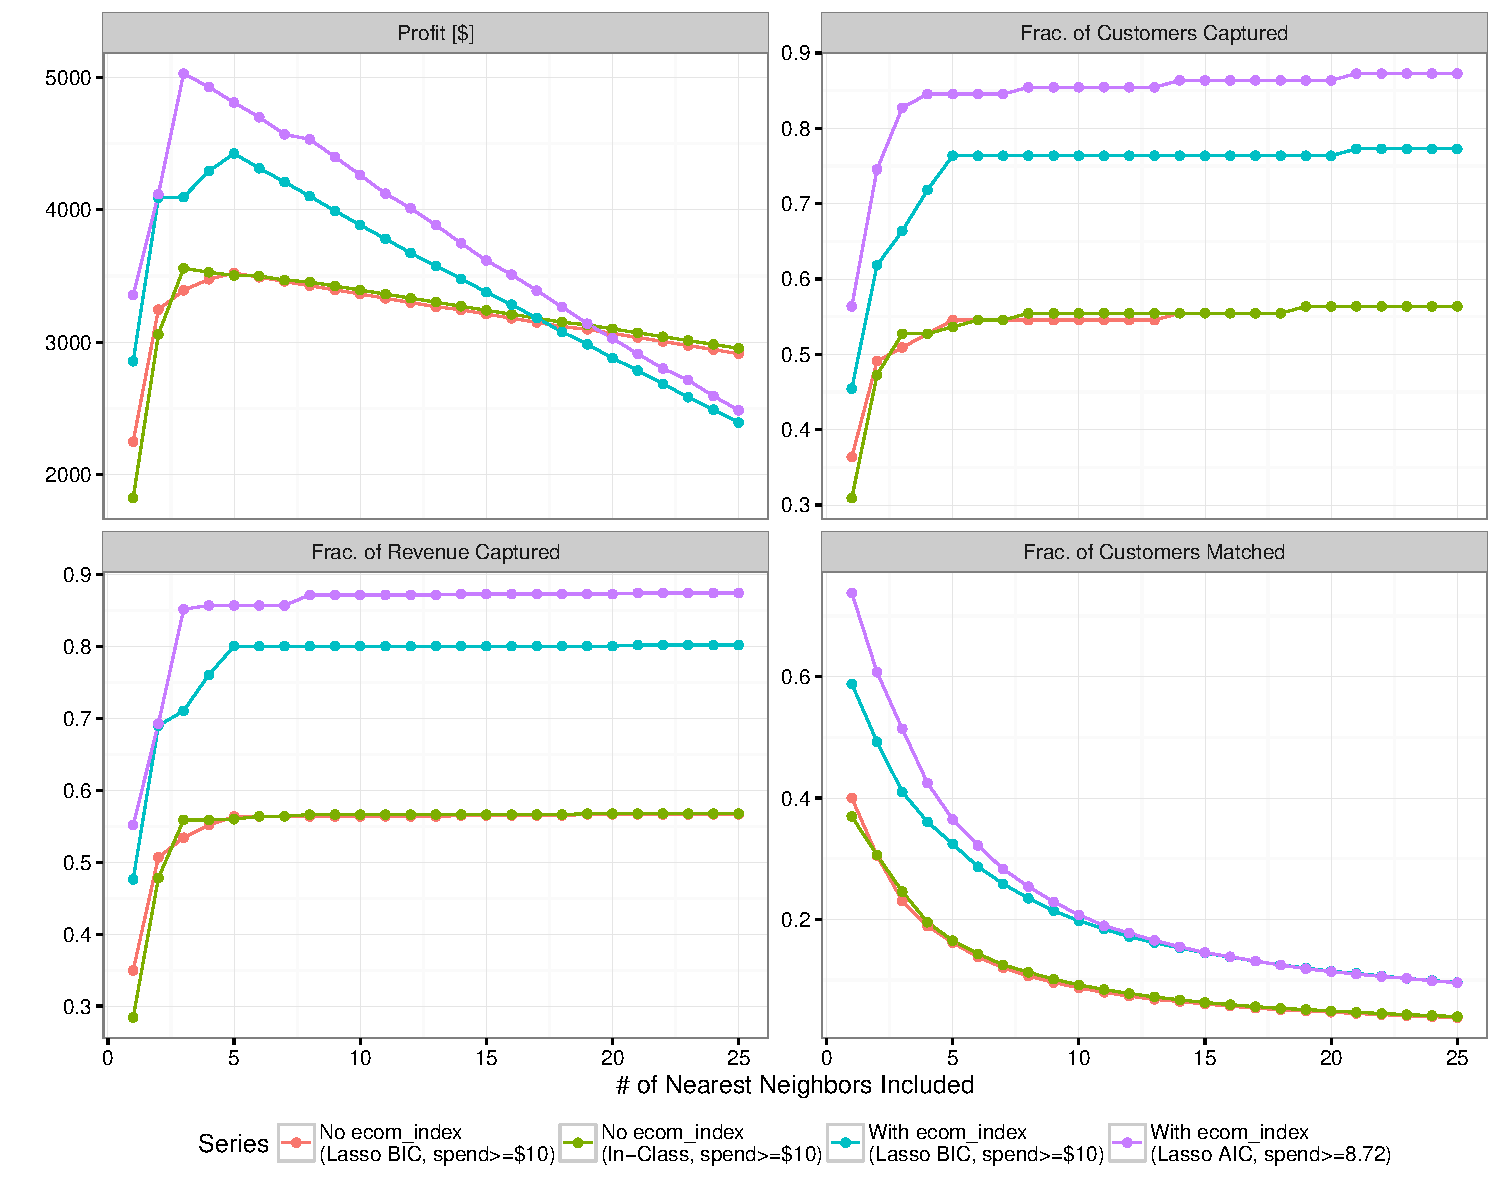
\includegraphics[scale=.75]{profits.pdf}
  \label{fig:profits}
\end{figure}


\section{Targeting the Entire Data Set (BC)} % Question 2

\clearpage
\section{Appendix}
% latex table generated in R 3.2.4 by xtable 1.8-0 package
% Tue Apr 12 09:38:48 2016
\begin{table}[ht]
\centering
\caption{Non-Zero Spend Quantiles} 
\label{tab:cutoffs}
\begin{tabular}{rrrr}
  \hline
Percentile & Spend & Percentile & Spend \\ 
  \hline
5 & 2.52 & 55 & 35.62 \\ 
  10 & 8.72 & 60 & 44.92 \\ 
  15 & 11.17 & 65 & 50.72 \\ 
  20 & 12.72 & 70 & 55.89 \\ 
  25 & 14.14 & 75 & 61.12 \\ 
  30 & 19.46 & 80 & 74.75 \\ 
  35 & 22.98 & 85 & 99.11 \\ 
  40 & 25.54 & 90 & 127.15 \\ 
  45 & 26.84 & 95 & 192.64 \\ 
  50 & 29.94 &  &  \\ 
   \hline
\end{tabular}
\end{table}


\end{document}

% \input{.tex}

% \begin{figure}[!htb]
%   \centering
%   \caption{}
%   \begin{subfigure}[b]{0.49\textwidth}
%     \caption{}
%     \includegraphics[width=\textwidth]{.pdf}
%     \label{fig:}
%   \end{subfigure}
%   \hfill
%   \begin{subfigure}[b]{0.49\textwidth}
%     \caption{}
%     \includegraphics[width=\textwidth]{.pdf}
%     \label{fig:}
%   \end{subfigure}
% \end{figure}

% \begin{figure}[!htb]
%   \centering
%   \caption{}
%   \includegraphics[scale=.5]{.pdf}
%   \label{fig:}
% \end{figure}